\documentclass{rapport}
\usepackage[utf8]{inputenc}
\usepackage[T1]{fontenc}
\usepackage[french]{babel}

\usepackage{pifont}
\usepackage{url}
\usepackage[hypertexnames=false,colorlinks, citecolor=red!60!green, linkcolor=blue!60!green, urlcolor=magenta]{hyperref}
\usepackage{float}
\usepackage{booktabs}
\usepackage{listings}
\usepackage{amsmath}
\usepackage{amssymb}
\usepackage{mathabx}
\usepackage{listings}

\usepackage{color}
\usepackage{tabularray}
\definecolor{Gin}{rgb}{0.894,0.933,0.894}
\definecolor{HalfandHalf}{rgb}{1,1,0.866}
\definecolor{Prim}{rgb}{0.929,0.866,0.929}

\theoremstyle{definition}
\newtheorem{definition}{Définition}

\theoremstyle{remark}
\newtheorem{lemme}{Lemme}

\theoremstyle{plain}
\newtheorem{example}{Example}

\theoremstyle{definition}
\newtheorem*{metric}{Métrique}

\theoremstyle{definition}
\newtheorem*{goal}{Objectif}

\theoremstyle{remark}
\newtheorem{remark}{Remarque}

\theoremstyle{definition}
\newtheorem*{Hypothesis}{Hypothèse}

\setlist[itemize,1]{label=\textbullet}
\setlist[itemize,2]{label=\textendash}
\setlist[itemize,3]{label=\textasteriskcentered}
\setlist[itemize,4]{label=\textperiodcentered}

\newcommand{\llbracket}{[\![}
\newcommand{\rrbracket}{]\!]}

\pagestyle{fancy}
\renewcommand{\sectionmark}[1]{\markboth{\thesection.\ #1}{}}
\fancyfoot{}
\fancyhead{}
\fancyhead[L]{\textsl{\leftmark}}
\fancyhead[R]{\textbf{\thepage}}
\setlength{\headheight}{23pt}

\lstset{
    basicstyle=\ttfamily\small,
    numbers=left,
    numberstyle=\tiny,
    breaklines=true,
}

\title{Affectation d'UE sous contraintes et équité\\Projet \emph{unica-course-allocation}}
\author{Promo Modélisation par des contraintes (2025-2026)}
\supervisor{Arnaud Malapert}
\date{}
\type{Projet}

\begin{document}

\maketitle

\begin{abstract}
Ce document constitue un rapport (version de travail) pour le projet \emph{unica-course-allocation} consacré à l'affectation des unités d'enseignement (UE) du Master Informatique.
Il présente le contexte et les objectifs, décrit les données disponibles, puis propose une formalisation des principales contraintes du problème.
L'ambition est de développer une méthode d'affectation explicable, qui améliore l'équité, tout en servant d'aide à la décision (comparaison et sélection de scénarios d'affectation).
Le document vise une longueur d'environ \textasciitilde{}20 pages (hors annexes).

Notez que les annexes ne sont pas nécessaires à la compréhension du sujet, mais constituent des éléments utiles pour une analyse du sujet en plus grande profondeur.
\end{abstract}

\clearpage
\tableofcontents
\clearpage

\section{Introduction et problématique}
\subsection{Description}
À l'université Côte d'Azur, les étudiants en master informatique structurent leur parcours chaque semestre en choisissant librement les matières qu'ils souhaitent suivre.
Le master est divisé en deux parcours : Informatique et IA. Peu importe leur spécialité, tous les étudiants suivent une sélection de cours/matières appelés << unité d'enseignement >> (UE).
Pour chaque parcours, certaines UE sont obligatoires et d'autres optionnelles. Au total, un étudiant suit entre 8 et 10 UEs.

Chaque UE dispose néanmoins d'un nombre de places limité. Comme différentes UE sont obligatoires dans certains parcours, le nombre de places proposées pour les autres parcours diminue également.
De plus, en raison d'incompatibilités entre certaines UE (conflit d'emploi du temps, par exemple), le choix des étudiants est limité.

Actuellement, l'université repose sur un système simple, compréhensible et facile à mettre en place pour l'attribution des places : << premier arrivé, premier servi >>.
Malheureusement, ce système engendre de multiples inégalités. En effet, les étudiants qui s'inscrivent en premier obtiennent toutes les UE qu'ils souhaitent, tandis que les derniers n'en obtiennent aucune.
À cela peuvent aussi s'ajouter des facteurs externes susceptibles de retarder le choix des étudiants (contraintes personnelles ou techniques, mauvaise manipulation, faible connexion Internet, etc.).
Le système actuel accentue également l'impact de ces facteurs sur le parcours final de l'étudiant.

Des étudiants et des professeurs, informés de cette problématique, lancent une initiative collective (IC) pour trouver une meilleure méthode d'affectation des UEs.

\subsection{Objectifs}
À travers une preuve de concept, l'IC devra répondre aux questions/consignes suivantes :
\begin{itemize}
    \item Le problème étant multicritère et multiagent, il n'existe pas d'affectation << optimale >> par nature. L'IC devra donc définir le concept d'<< affectation équitable >> et trouver un moyen de l'évaluer quantitativement.
    \item Proposez un processus simple à mettre en place, de préférence compréhensible et explicable, permettant d'améliorer le système d'affectation des UEs.
    \item Proposez une preuve de concept flexible à d'autres paramètres (nombre de cours, d'étudiants, de parcours/spécialités, de places, nombre de cours obligatoires, etc.).
    \item Présentez vos résultats de manière à ce que votre système soit \textbf{facilement compréhensible} et \textbf{scientifiquement cohérent}.
\end{itemize}
\textbf{Note 1 :} \underline{\textit{Idéalement}}, le système proposé doit être simple (processus, algorithmes, etc.), facile à comprendre, à vulgariser et à exploiter, mais aussi compréhensible, explicable et << intègre >> (il ne doit pas être possible de le détourner facilement pour obtenir un avantage par rapport aux autres étudiants).

\begin{definition}[Équité (définition opérationnelle)]
    Dans ce rapport, nous proposons pour commencer une définition simple de l'équité, que nous développerons au fur-et-à-mesure de celui-ci. Ainsi, nous qualifierons, dans un premier temps, d'affectation << équitable >> toutes affectations (i) respectant les contraintes du problème énoncé, (ii) garantissant un niveau de satisfaction << acceptable >> pour l'ensemble des étudiants (éviter les situations très défavorisées), (iii) limitant les écarts de satisfactions entre les étudiants, (iv) tout en restant compatible avec une interprétation simple par les responsables de formation.
\end{definition}

\subsection{Organisation du rapport}
Ce rapport, volontairement concis (\textasciitilde{}20 pages hors annexes), couvre l'architecture globale du projet :
\begin{figure}[H]
    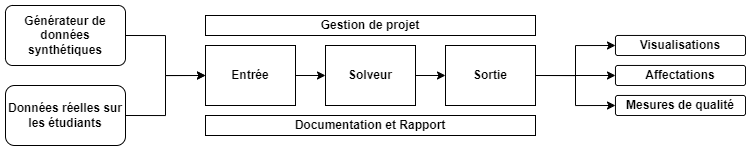
\includegraphics[width=\textwidth]{img/Project Flow Diagram.png}
    \caption{Architecture globale du projet}
\end{figure}

L'entrée traite de la récupération, de la gestion et de la transformation des données pour leur exploitation ; le solveur résout le problème d'affectation ; enfin, la sortie gère la visualisation et l'évaluation des affectations.
Dans ce rapport, après l'introduction du contexte et des objectifs, nous présentons le format des données, les contraintes que nous exploiterons, les métriques et mesures de qualité définissant une affectation << équitable >>, les processus et méthodes employés pour les obtenir, ainsi que les visualisations utiles pour comparer différentes affectations et soutenir une décision.


\section{Données}\label{sec:Data}
\subsection{Données disponibles}
Pour mener à bien ce projet, l'IC dispose des informations suivantes :
\begin{itemize}
  \item La liste complète des UEs obligatoires et optionnelles pour chaque parcours, ainsi que le nombre de places disponibles (hors places réservées pour les UE obligatoires) ;
    \item L'EdT du semestre, afin d'observer les potentiels conflits entre les UEs ;
    \item La liste des préférences de chaque étudiant pour chaque UE proposée, le nombre d'UE qu'il souhaite suivre et sa spécialité.
\end{itemize}

Notes :
\begin{itemize}
    \item Certaines UE externes au processus principal d'affectation peuvent être considérées comme ayant une capacité << illimitée >>,
    \item Toutes les UEs non obligatoires dans un parcours sont considérées comme optionnelles.
\end{itemize}

\subsection{Format des données}
Soit $n$ le nombre d'étudiants, $m$ le nombre d'UE et $p$ le nombre de parcours.
On note $N = \llbracket 1,n \rrbracket$, $M = \llbracket 1,m \rrbracket$ et $P = \llbracket 1,p \rrbracket$ les ensembles d'indices.
La notation $\llbracket a,b \rrbracket$ désigne l'ensemble des entiers de $a$ à $b$ inclus.

\subsubsection{Entrée}
\begin{itemize}
    \item \textbf{Unités d'Enseignements :}
    \begin{itemize}
        \item $c_j \in \mathbb{N}$ : la capacité de l'UE $j \in M$.
        \item $I^c_{j,j'} \in \{0,1\}$ : indicatrice d'incompatibilité entre deux UE $(j,j') \in M^2$ (1 si incompatibles, 0 sinon).
    \end{itemize}

    \item \textbf{Parcours :}
    \begin{itemize}
        \item $m\!\min_k \in \mathbb{N}^*$ : le nombre minimum d'UE optionnelles à suivre dans le parcours $k \in P$.
        \item $m_{j,k} \in \{0,1\}$ : indicatrice \og l'UE $j \in M$ est obligatoire dans le parcours $k \in P$ \fg{}.
    \end{itemize}

    \item \textbf{Étudiants :}
    \begin{itemize}
        \item $m\!\max_i$ : le nombre maximum d'UE souhaité par l'étudiant $i \in N$.
        \item $p_i \in P$ : le parcours suivi par l'étudiant $i \in N$.
        \item $r_i : M \to \mathbb{R}^{+}$ : une fonction de rang (par la méthode des rangs moyens) décrivant les préférences de l'étudiant $i$, telle que plusieurs UE peuvent avoir le même rang, que les rangs soient consécutifs, que la somme des rangs soit égale pour tous les étudiants et que le premier rang soit occupé par les UE obligatoires (si applicable).
    \end{itemize}
\end{itemize}

\subsubsection{Sortie}
\begin{itemize}
    \item $A_{i,j}$ : une affectation d'UE pour l'étudiant $i \in N$ ; 1 si l'UE $j \in M$ est affectée, 0 sinon.
\end{itemize}

\subsubsection{Contraintes}
\begin{itemize}
    \item[] \textbf{(C1)} \og Pour chaque UE, la somme des affectations pour celle-ci ne dépasse pas sa capacité \fg{} :
    \[
    \forall j \in M : \sum_{i \in N} A_{i,j} \le c_j
    \]

    \item[] \textbf{(C2)} \og Une affectation ne peut accorder que des UE compatibles \fg{} :
    \[
    \forall i \in N,\ \forall (j,j') \in M^2\ \text{tels que}\ I^c_{j,j'} = 1 : A_{i,j} + A_{i,j'} \le 1
    \]

    \item[] \textbf{(C3)} \og Un étudiant inscrit dans un parcours $p$ doit se voir attribuer toutes les UE obligatoires du parcours $p$ \fg{} :
    \[
    \forall i \in N,\ \forall j \in M : A_{i,j} \ge m_{j,p_i}
    \]

    \item[] \textbf{(C4)} \og Un étudiant doit recevoir une affectation de 8 à 10 UE \fg{} :
    \[
    \forall i \in N : 8 \le \sum_{j \in M} A_{i,j} \le 10
    \]

    \item[] \textbf{(C5)} \og Un étudiant peut recevoir au maximum le nombre de UE qu'il a demandé \fg{} :
    \[
    \forall i \in N : \sum_{j \in M} A_{i,j} \le m\!\max_i
    \]
\end{itemize}

\paragraph{Note.}
$\mathbf{1}_{a=b}$ est la fonction indicatrice définie par 1 si $a=b$ et 0 sinon. Les quantités $p_i$, $m_{j,k}$, $I^c_{j,j'}$, $c_j$ et $m\!\max_i$ sont des données d'entrée (paramètres), tandis que $A_{i,j}$ est la variable de décision.

\begin{example}[Exemple du format de sortie]
    Considérons $n=2$ étudiants ($N=\llbracket 1,2\rrbracket$), $m=3$ UE ($M=\llbracket 1,3\rrbracket$) et $p=2$ parcours ($P=\llbracket 1,2\rrbracket$).
    On fixe les capacités $(c_1,c_2,c_3)=(1,2,1)$ et une incompatibilité unique $I^c_{1,3}=I^c_{3,1}=1$ (les autres valent 0). Le parcours de l'étudiant 1 est $p_1=1$ et celui de l'étudiant 2 est $p_2=2$.
    Si l'UE 2 est obligatoire dans le parcours 1 (donc $m_{2,1}=1$) et aucune UE n'est obligatoire dans le parcours 2, alors l'affectation
    \begin{center}
        \begin{tabular}{c|ccc}
            & $j=1$ & $j=2$ & $j=3$ \\
            \hline
            $i=1$ & 0 & 1 & 0 \\
            $i=2$ & 1 & 0 & 0
        \end{tabular}
    \end{center}
    satisfait (C1) (capacités), (C2) (pas de couple incompatible attribué à un même étudiant) et (C3) (UE obligatoire du parcours 1 attribuée à l'étudiant 1).
\end{example}


\section{Métriques d'évaluations et de comparaisons}\label{sec:Metric}

Dans le cadre de ce projet, il est important de pouvoir évaluer et comparer plusieurs instances d'affectation d'étudiants.
Sans cela, nous serions en effet incapables de mesurer une potentielle amélioration du système actuellement exploité, mais aussi de vérifier l'existence d'éventuels biais dans les affectations, et donc d'établir si une affectation est << équitable >>.

Pour atteindre cet objectif, nous devons développer des métriques et des indicateurs adaptés au problème.
Dans ce rapport, nous nous concentrons sur les métriques vectorielles contenant une valeur pour chaque entité mesurée, mais aussi sur d'autres indicateurs nous permettant d'évaluer les biais potentiels d'une affectation.

\begin{remark}
    Ce document concentre les informations les plus importantes, mais un important travail de réflexion sur les métriques, les éventuelles alternatives et les biais induits a été mené. Il est disponible sous la forme d'une annexe (\textbf{\textit{Annexe I - Brouillon et Réflexions sur les Métriques}}), dont cette partie constitue un résumé.
\end{remark}

Dans la suite de cette section, nous présentons certaines des métriques développées, ainsi que leurs avantages et leurs inconvénients.
Avant cela, nous devons toutefois définir plusieurs notions :

\begin{definition}[Produit de Schur]
    Soit $X$ et $Y$ deux matrices de même dimension dans $\mathbb{R}_{n,m}$, nous définissons le produit de Schur $\odot$
    comme l'opération qui associe à $X$ et $Y$ la matrice $Z$ tel que $\forall (i,j)\in N\times M:z_{i,j}=x_{i,j}\cdot y_{i,j}$. Ou plus graphiquement :
    $$
    Z = X\odot Y = \begin{bmatrix}
        x_{0,0} & \cdots & x_{0,m} \\
        \vdots & \ddots & \vdots \\
        x_{n,0} & \cdots & x_{n,m}
    \end{bmatrix} \odot \begin{bmatrix}
        y_{0,0} & \cdots & y_{0,m} \\
        \vdots & \ddots & \vdots \\
        y_{n,0} & \cdots & y_{n,m}
    \end{bmatrix} = \begin{bmatrix}
        x_{0,0}\cdot y_{0,0} & \cdots & x_{0,m}\cdot y_{0,m} \\
        \vdots & \ddots & \vdots \\
        x_{n,0}\cdot y_{n,0} & \cdots & x_{n,m}\cdot y_{n,m}
    \end{bmatrix}
    $$
\end{definition}

\begin{definition}[Matrice des rangs d'affectation]
    Soit $A_{i,j}\in\{0,1\}_{n,m}$ la matrice représentant l'affectation accordée à l'étudiant $i\in N$ pour l'UE $j\in M$.
    Soit $R_{i,j}\in\mathbb{R}^{+}_{n,m}$ la matrice représentant les rangs accordés par l'étudiant $i\in N$ pour l'UE $j\in M$, nous
    définissons la matrice des rangs d'affectation $U_{i,j} = A_{i,j} \odot R_{i,j}$ comme la matrice des rangs des UE effectivement affectés à l'étudiant $i$.
\end{definition}

\begin{example}\label{ex:running1}
    Dans le cadre de ce rapport, nous allons développer un exemple fictif que nous exploiterons tout au long de l'étude à des fins d'illustration.
    Pour cet exemple, nous aurons cinq étudiants : Sophie et Pierre, suivant le parcours IA, puis Hugo, Axel et Sabine, suivant le parcours Informatique.
    Il y a 4 UEs : AI est obligatoire en IA, Code est obligatoire en Informatique, Éco et Droit sont optionnels. Chaque cours dispose de quatre places (places réservées incluses).
    Un étudiant doit choisir entre deux et trois UEs. Voici les préférences de chaque étudiant, ainsi que le nombre d'UEs qu'ils souhaitent prendre :

    $$
    \begin{aligned}
    R_{i,j} &=
        \begin{bmatrix}
            \text{UEs} & \text{AI} & \text{Code} & \text{Éco} & \text{Droit}\\
            \text{Sophie} & 1 & 2 & 3 & 4\\
            \text{Pierre} & 1 & 2 & 3 & 4\\
            \text{Hugo} & 2 & 1 & 3 & 4\\
            \text{Axel} & 2 & 1 & 4 & 3\\
            \text{Sabine} & 2 & 1 & 3 & 4
        \end{bmatrix}
    \quad
    m\!\max\!_i &=
        \begin{bmatrix}
            \text{UEs} & m\!\max_i\\
            \text{Sophie} & 2\\
            \text{Pierre} & 3\\
            \text{Hugo} & 3\\
            \text{Axel} & 3\\
            \text{Sabine} & 3
        \end{bmatrix}
    \end{aligned}
    $$
    Usant d'une affectation arbitraire, voici les affectations reçus et la matrice des rangs d'affectation correspondante :
    $$
    \begin{aligned}
    A_{i,j} &=
        \begin{bmatrix}
            \text{UEs} & \text{AI} & \text{Code} & \text{Éco} & \text{Droit}\\
            \text{Sophie} & 1 & 1 & 0 & 0\\
            \text{Pierre} & 1 & 0 & 1 & 1\\
            \text{Hugo} & 1 & 1 & 1 & 0\\
            \text{Axel} & 1 & 1 & 0 & 1\\
            \text{Sabine} & 0 & 1 & 1 & 1
        \end{bmatrix}
    \quad
    U_{i,j} &=
        \begin{bmatrix}
            \text{UEs} & \text{AI} & \text{Code} & \text{Éco} & \text{Droit}\\
            \text{Sophie} & 1 & 2 & 0 & 0\\
            \text{Pierre} & 1 & 0 & 3 & 4\\
            \text{Hugo} & 2 & 1 & 3 & 0\\
            \text{Axel} & 2 & 1 & 0 & 3\\
            \text{Sabine} & 0 & 1 & 3 & 4
        \end{bmatrix}
    \end{aligned}
    $$
    Grâce à celle-ci, nous pouvons donc voir que tous les étudiants se sont vu attribuer leurs UEs obligatoires, et que Sabine et Pierre n'ont pas obtenu leur deuxième choix.
    Nous pouvons également constater que les cours AI et Code sont complets.
\end{example}

Maintenant que nous avons introduit la matrice des rangs d'affectation, nous pouvons présenter les métriques vectorielles que nous utiliserons dans ce projet.
Toutefois, avant cela, nous devons réfléchir à la nature des données et à leurs biais intrinsèques.

\subsection{Biais de type I}
Dans la plupart des mesures auxquelles nous souhaiterions recourir (moyenne, somme, écart-type, etc.), nous constatons tout d'abord que nous travaillerons sur des rangs qui, par nature, augmentent avec le nombre d'entités classées.
De plus, nous observons que chaque étudiant dispose d'une certaine liberté dans le choix du nombre d'UEs. Si cela est bénéfique pour l'étudiant, cela rend toutefois propice l'apparition de biais dans nos futures mesures.

Ainsi, si un étudiant $E_1$ choisit 9 UEs et un autre $E_2$ en choisit 7, $E_1$ se verra octroyer des rangs supplémentaires dans la matrice d'affectation des rangs (pour la huitième et la neuvième UE) ; or, par nature, ces rangs sont plus élevés que le septième rang qui lui a été attribué.
Des métriques intéressantes, comme le dernier rang, la somme ou la moyenne des rangs, ou encore l'écart-type, se voient donc artificiellement augmentées. Comme $E_2$ ne se voit pas attribuer de huitième et de neuvième rang, il aura en général des valeurs plus faibles pour les métriques citées que $E_1$.

Bien que cette remarque semble anodine, elle pose en réalité un véritable problème, car elle s'étend aux optimisations que nous chercherons à effectuer pour obtenir la << meilleure >> affectation possible.
En effet, nous cherchons généralement à minimiser une métrique sur les rangs ; ainsi, $E_1$ aura une valeur plus élevée pour cette métrique et sera probablement priorisé par rapport à $E_2$, même si celui-ci pourrait avoir une moins bonne affectation en général.
Nous désignerons ce biais comme un biais de <<\textbf{Type I}>> (un biais, dit de Type II, existe également sur des instances particulières ; voir l'Annexe I pour plus d'informations).
Pour réduire ce biais au maximum, nous devons tout d'abord mieux préciser la nature des UEs.

\begin{definition}
    Soit $\text{aSet(i)}\subseteq M=\arg_j\left\{\mathbf{1}_{A_{i,j}=1}\right\}$, l'ensemble, ordonné par rangs, des UEs affectés à un étudiant $i\in N$, nous pouvons distinguer trois types d'UEs :
    les UEs obligatoires pour l'étudiant en raison du parcours que l'on notera $\text{mSet(i)}$,
    celles optionnelles permettant d'atteindre le quota minimum d'UE pour passer le semestre $\text{oSet}(i)$
    et les UEs facultatives définis par $\text{fSet(i)} = \text{aSet}(i)\setminus[\text{mSet}(i)\cup\text{oSet}(i)]$.
    Attention, les trois ensembles sont disjoints.
\end{definition}
Étant donné que le nombre minimum d'UE requis pour passer le semestre pour chaque étudiant peut être obtenu par $m_{\min}(i)=\#\text{oSet}(i)+m\!\min_{p_i} \forall i \in N$,
nous pouvons montrer que le nombre d'UE minimum pour passer le semestre $m_{\min}(i)$ est constant pour tous les étudiants d'un même parcours. En pratique, nous pourrons émettre l'hypothèse que ce nombre d'UE
est égal peu importe les parcours.

\begin{example}\label{ex:running2}
    En se basant sur l'exemple~\ref{ex:running1}, nous reprenons nos étudiants : Sophie, Pierre, Hugo, Axel et Sabine. Voici l'ensemble ordonné des affectations, des affectations obligatoires, optionnelles et facultatives pour chacun d'entre eux :
    $$
    \begin{bmatrix}
        \text{Étudiant} & \text{Sophie} & \text{Pierre} & \text{Hugo} & \text{Axel} & \text{Sabine}\\
        \text{aSet}(i) & \{\text{AI, Code}\} & \{\text{AI, Éco, Droit}\} & \{\text{Code, AI, Éco}\} & \{\text{Code, AI, Droit}\} & \{\text{Code, Éco, Droit}\}\\
        \text{mSet}(i) & \{\text{AI}\} & \{\text{AI}\} & \{\text{Code}\} & \{\text{Code}\} & \{\text{Code}\}\\
        \text{oSet}(i) & \{\text{Code}\} & \{\text{Éco}\} & \{\text{AI}\} & \{\text{AI}\} & \{\text{Éco}\}\\
        \text{fSet}(i) & \emptyset & \{\text{Droit}\} & \{\text{Éco}\} & \{\text{Droit}\} & \{\text{Droit}\}
    \end{bmatrix}
    $$
    Ici, nous pouvons voir la nature de << tiroir >> de ces catégories : nous remplissons d'abord l'ensemble des UEs obligatoires, puis les UEs optionnelles, et enfin les UEs facultatives, s'il y en a.
\end{example}

Dans notre cas, où nous émettons l'hypothèse que le nombre d'UE dans l'union de $\text{mSet}$ et de $\text{oSet}$ est identique pour chaque étudiant et parcours (ce qui est bien le cas dans notre master, mais attention, ce n'est pas forcément le cas dans le cadre général), nous disposons maintenant d'une borne fixe sur le nombre d'UE plutôt que d'une borne variant selon les souhaits des étudiants.
Ainsi, les étudiants étant placés à la même enseigne, le biais de Type I n'a plus d'effet si nous calculons nos métriques sur l'ensemble des affectations non facultatives.

À noter néanmoins que cela a une forte implication : \textbf{Les UEs facultatives sont moins importantes que les UEs non facultatives}.
Nous pouvons donc nous permettre une moins bonne affectation des UEs facultatives, que l'étudiant pourra abandonner sans conséquences, si cela nous permet d'avoir une meilleure affectation des UEs obligatoires et optionnelles, que l'étudiant ne pourra pas abandonner s'il veut valider son semestre.

Maintenant que cela est dit, nous pouvons enfin passer à nos métriques vectorielles.

\subsection{Métriques vectorielles}
\begin{metric}[Dernier rang non facultatif affecté]
    Définie pour les étudiants uniquement, le dernier rang non facultatif affecté correspond pour chaque étudiant $i$ au rang maximum des $m_{\min}(i)$ UEs au rang le plus faible.
    Elle se formalise ainsi :
    $$
        \forall i\in N : \text{lastMandatoryRank}(i) = \max_{j\in \text{mSet}(i)\cup\text{oSet}(i)} U_{i,j}
    $$
    En prenant le dernier rang des UEs requises pour valider le semestre, cette métrique est intuitive, compréhensible et simple à calculer, tout en fournissant une borne supérieure sur les rangs affectés (ce qui peut être utile pour des minimisations).
    Malheureusement, elle ne prend pas en compte la distribution des rangs inférieurs.
    Autrement dit, un étudiant peut se voir attribuer un dernier rang élevé, mais avoir des UEs de rangs faibles pour les autres affectations ; inversement, un étudiant peut avoir un dernier rang moyen, mais voir ses autres affectations très concentrées autour de cette borne, ce qui rend l'affectation insatisfaisante pour lui.
    Nous devons donc trouver une autre métrique qui tienne compte de cette distribution, ne serait-ce qu'implicitement.
\end{metric}

\begin{metric}[Somme des rangs non facultatifs]
    Définie pour les étudiants, la somme des rangs non facultatifs correspond à la métrique qui additionne les rangs de l'ensemble des UEs non facultatives affectées à chaque étudiant.
    Elle se formalise ainsi :
    $$
        \forall i\in N : \text{correctedRankSum}(i) = \sum_{j\in M} U_{i,j}-\sum_{j\in\text{fSet}(i)} U_{i,j}
    $$
    Cette métrique présente plusieurs avantages.
    Premièrement, elle est facilement interprétable : plus la valeur est élevée, plus l'étudiant est lésé ; plus la valeur est faible, meilleure est la satisfaction de l'étudiant.
    Deuxièmement, cette métrique est rapide et simple à calculer, et permet de prendre en compte la distribution sous-jacente des rangs non facultatifs affectés de manière implicite.
    Enfin, elle reste intuitive, simple à accepter, à comprendre et à expliquer, ce qui rend le système plus abordable pour les exploitants.
\end{metric}

\begin{example}\label{ex:running3}
    Dans la continuité des exemples précédents, nous allons maintenant calculer les métriques citées précédemment sur nos étudiants :
    $$
    \begin{bmatrix}
        \text{Étudiant} & \text{Sophie} & \text{Pierre} & \text{Hugo} & \text{Axel} & \text{Sabine}\\
        \text{lastMandatoryRank}(i) & 2 & 3 & 2 & 2 & 3\\
        \text{correctedRankSum}(i) & 3 & 4 & 3 & 3 & 4\\
    \end{bmatrix}
    $$
    Nous observons ici que les dernières UE affectées n'ont pas eu d'impact sur la somme des rangs non facultatifs ou sur le dernier rang non facultatif. Cela donne dans notre cas des valeurs similaires pour chacun des étudiants, ce qui est une bonne chose et constitue une première piste pour la notion d'équité, que nous n'avons pas encore définie formellement.
    Nous pouvons également constater l'intérêt de prendre en compte ces métriques corrigées du biais de Type I plutôt que les métriques non corrigées. Ainsi, dans cet exemple, Sophie aurait toujours obtenu une somme de 3, tandis que Hugo aurait obtenu une somme de 6, alors que leur affectation concernant les UEs non facultatives est sensiblement identique.
\end{example}

À partir de là, il peut également être intéressant d'établir une moyenne et un écart-type afin de mieux comprendre la distribution des rangs non facultatifs affectés ; toutefois, cela alourdirait considérablement l'analyse des affectations pour l'opérateur (si l'on considère que la somme et la moyenne sont la même chose, à une constante multiplicative près). Malgré tout, cela reste intéressant d'un point de vue statistique, et ces métriques sont implémentées aux côtés d'autres métriques (voir l'Annexe I pour plus de détails).

Les métriques développées plus haut sont directement utilisables dans un solveur linéaire, mais il existe aussi des métriques non linéaires qui peuvent être intéressantes pour leur interprétation. C'est ce que nous allons voir maintenant.

\begin{definition}
    Soit $X$ une variable aléatoire et $x\in]0,1[$. Le quantile d'ordre $x$ de la distribution de $X$, noté $Q_x$, est définit par : $Q_x = \min\{y\in\mathbb{R} : \mathbb{P}[X\le y]\ge x\}$.
    Ainsi, le premier quartile $Q_1 \equiv Q_{0.25}$, correspond à la valeur $y$ tel que 25\% de la population est en dessous de $y$.
    De même, la médiane (ou deuxième quartile) $Q_2\equiv Q_{0.5}$ correspond à la valeur $y$ tel que la moité de la population se trouve en dessous de cette valeur.
    Enfin, le troisième quartile $Q_3\equiv Q_{0.75}$ équivaut à la valeur $y$ tel que les trois quarts de la population se trouve en de dessous de $y$.
\end{definition}

\begin{metric}[Médianes et Quartiles des rangs non-facultatifs affectés]
    Définie pour les étudiants, le premier, le deuxième et le troisième quartile des rangs non facultatifs sont formalisés ainsi (par abus de langage) :
    $$
    \forall i\in N : Q_{0.25|0.5|0.75}(i) = \min\{y : \mathbb{P}[\text{aSet}(i)\setminus\text{fSet}(i)\le y]\ge 0.25|0.5|0.75\}
    $$
    Bien que non linéaires et plus compliquées à calculer que la moyenne (en pratique, il existe souvent une fonction, dans le langage de programmation utilisé, permettant de les calculer simplement), cette famille de métriques offre de nombreux avantages.
    En effet, elle permet de disposer d'une mesure de centralité résistante aux valeurs extrêmes (voir le biais de Type II dans l'Annexe I pour plus de détails), d'une interprétation intéressante, notamment la médiane qui permet de séparer 50\% de la population, mais aussi de prendre en compte la distribution sous-jacente grâce à l'analyse des quantiles.
    Par exemple, si $Q_1$ est élevé par rapport au rang minimum, nous savons d'emblée que la distribution est étalée sur la gauche (ce qui est une mauvaise chose).
    De même, si $Q_3$ est faible, nous observons que la distribution est étalée sur la droite (ce qui est une bonne chose).

    Dans les faits, nous n'irons généralement pas aussi loin et nous contenterons de l'interprétation de la médiane.
\end{metric}

À noter que, comme pour la moyenne, la médiane possède une mesure de dispersion appelée écart interquartile (ou $\text{IQR}(i) = Q_3(i) - Q_1(i)$).
Contrairement à l'écart-type, celui-ci dispose d'une interprétation naturelle qui permet d'expliciter la dispersion des 50\% de la population autour de la médiane.
C'est pour cette raison que nous le mentionnons tout de même.

\begin{example}\label{ex:running4}
    Encore une fois, comme pour l'exemple~\ref{ex:running3}, nous allons calculer les nouvelles métriques pour nos étudiants.
    $$
    \begin{bmatrix}
        \text{Étudiant} & \text{Sophie} & \text{Pierre} & \text{Hugo} & \text{Axel} & \text{Sabine}\\
        Q_2(i)          & 1.5 & 2 & 1.5 & 1.5 & 2\\
        \text{IQR}(i)   & 1   & 2 & 1   & 1   & 2\\
    \end{bmatrix}
    $$
    Dans notre petit exemple, les notions de médiane et d'IQR perdent un peu de leur sens, surtout si l'on considère qu'une correction de continuité est généralement effectuée pour atteindre les quantiles désirés via Python ou tout autre langage de programmation.
    Malgré tout, nous pouvons dire à partir de ces données qui ont eu la moins bonne affectation : Pierre et Sabine.
    En effet, ces derniers ont obtenu la médiane la plus élevée : 50\% des UEs attribuées ont un rang supérieur à 2, et leur IQR est élevé (dans ce contexte), ce qui signifie que leurs rangs sont plus dispersés que ceux des autres étudiants.
    Idéalement, nous chercherions une médiane et un IQR faibles sur les rangs non-facultatifs.
\end{example}

\subsection{Indicateurs de qualité et d'équité}
Les métriques que nous développons peuvent servir à plusieurs fins, notamment la réduction des biais, l'optimisation des affectations en tant qu'heuristique, et bien sûr l'évaluation des affectations.
Notre objectif est d'atteindre une notion d'<< équité >> que nous allons enfin définir.

\begin{definition}[Équité]
    Selon le Larousse, l'équité se définit comme << la qualité consistant à attribuer à chacun ce qui lui est dû, conformément aux principes de la justice naturelle ; impartialité >>.
    En d'autres termes, nous chercherons à ce que les affectations ne soient influencées que par le choix des étudiants. L'objectif est donc de faire en sorte qu'aucun étudiant ne soit avantagé par rapport à un autre lors de l'affectation des UEs.

    Concrètement, sur le dernier rang non facultatif affecté, cela se traduirait par << le dernier rang non facultatif affecté à un étudiant est le plus faible possible (optimisation) et similaire à celui des autres étudiants (minimiser les différences) >>.
\end{definition}

Cette définition et cet exemple montrent donc que les métriques vectorielles permettent généralement d'attribuer un score à l'affectation d'un étudiant, tandis qu'une agrégation de ces métriques (voir l'Annexe I pour plus de détails) permet d'évaluer la notion d'équité (par exemple, des médianes faibles et un écart interquartile faible, ou des moyennes faibles et des écarts-types faibles).

Comme mentionné précédemment, la notion d'équité peut être définie en partie par des métriques, mais elle prend également en compte des facteurs plus indirects, tels que la question de savoir si un groupe d'étudiants est plus favorisé qu'un autre. À partir de maintenant, nous allons examiner trois méthodes complémentaires pour évaluer cette équité.
Commençons directement par une agrégation : le coefficient de Gini.

\subsubsection{Le coefficient de Gini}
\begin{metric}[Coefficient de Gini]
    Soit $m_v$ une métrique vectorielle numérique quelconque de longueur $\#m_v$. Soit $\widebar{m_v}$ la moyenne calculée sur $m_v$, nous définissons le coefficient de Gini ainsi :
    $$
        \text{Gini}(m_v) = \frac{\sum_{i=1}^{\#m_v}\sum_{j=1}^{\#m_v}\left|x_i-x_j\right|}{2\left[\#m_v\right]^2\widebar{m_v}}
    $$
    Initialement très utilisé pour comparer la répartition des richesses, cet indice peut aussi être utilisé dans un cadre général comme mesure d'inégalité.
    Bien que complexe à calculer, son interprétation reste simple : si le coefficient de Gini approche 0, alors toutes les valeurs de la métrique vectorielle sont identiques ; dans le cas contraire, si l'indice s'approche de 1, alors un individu possède l'intégralité des richesses tandis que les autres ne possèdent rien.

    Dans notre contexte, si l'on utilise la somme des rangs non facultatifs affectés, un coefficient de Gini proche de 0 indique une égalité parfaite des affectations.
    Attention toutefois, dans ce contexte, un coefficient de 1 n'indique pas qu'un individu est grandement bénéficiaire du système au détriment des autres, mais plutôt que, s'il existait, il serait certainement le plus lésé.
    En d'autres termes, si le coefficient de Gini est proche de 1 sur une métrique telle que la somme des rangs, alors la personne concentrant les << richesses >> serait en réalité une personne dont l'affectation a été créée de manière intentionnellement mauvaise afin de faire bénéficier le reste du groupe de son << sacrifice >>.
\end{metric}

\begin{example}\label{ex:running5}
    Toujours dans la continuité des exemples, calculons l'indice de Gini pour les métriques calculés dans l'exemple~\ref{ex:running3} sur l'affectations des UEs de Sophie, Pierre, Hugo, Axel et Sabine.
    Nous avons $\widebar{m_\text{sum}} = \frac{3+4+3+3+4}{5}=3.4$ et $\widebar{m_\text{last}} = \frac{2+3+2+2+3}{2.4}$, avec $\#m_{\text{sum}} = \#m_{\text{sum}} = 5$.
    Ainsi, nous avons :
    $$
    \text{Gini}(m_{\text{sum}}) = \frac{3\cdot\left(3\cdot|3-3|+2\cdot|3-4|\right)+2\cdot\left(3\cdot|4-3|+2\cdot|4-4|\right)}{2\cdot5^2\cdot3.4} = \frac{12}{170} \approxeq 0.071
    $$
    et :
    $$
    \text{Gini}(m_{\text{last}}) = \frac{3\cdot\left(3\cdot|2-2|+2\cdot|2-3|\right)+2\cdot\left(3\cdot|3-2|+2\cdot|3-3|\right)}{2\cdot5^2\cdot2.4} = \frac{12}{120} = 0.1
    $$
    Comme nous pouvions nous y attendre, l'indice de Gini pour les deux métriques est faible et s'approche de 0, ce qui indique que l'affectation est équitable.
\end{example}

\begin{remark}[Optimalité et Équité]
    Attention, l'équité n'implique pas l'optimalité. Ainsi, il est possible d'avoir une affectation équitablement mauvaise pour tous.
    La réciproque est également vraie : en fonction des métriques utilisées, nous pourrions avoir une affectation optimale (généralement bonne), mais inéquitable pour un groupe discriminé.
\end{remark}

Bien que l'indice de Gini soit intéressant pour détecter les affectations lésant fortement un ou plusieurs étudiants, il ne permet pas de conclure sur l'affectation de manière globale.
Pour cela, nous pouvons utiliser un autre indicateur basé sur le front de Pareto.

\subsubsection{Pareto en tant que mesure d'équité}
Dans notre situation, où nous cherchons à offrir une affectation à chaque étudiant, plusieurs solutions plus ou moins bonnes coexistent.
Il est parfois possible de passer d'une solution à une autre en échangeant l'affectation d'un étudiant avec celle d'un autre.
À partir de là, nous pouvons définir l'équité d'une affectation comme l'absence de tels échanges.

\begin{definition}[Échange technique]
    Soit deux étudiants différents $\left(i_a,i_b\right)\in N^2_{a\ne b}$ où $n$ est le nombre d'étudiant.
    Nous définissons un << échange technique >> comme un échange des affectations de $i_a$ et de $i_b$, tel que la contraintes des UEs obligatoires est respectée, plus formellement : $\left[\text{mSet}(i_a)\subseteq\text{aSet}(i_b)\right] \land \left[\text{mSet}(i_b)\subseteq\text{aSet}(i_a)\right]$
    et que le nombre d'UE demandé par chacun des étudiant ne soit pas dépassé $m\!\max_{i_a}\ge\#\text{aSet}(i_b)\land m\!\max_{i_b}\ge\#\text{aSet}(i_a)$.
    On notera le prédicat $i_a\stackrel{T}{\longleftrightarrow} i_b$ valant 0 s'il n'existe pas d'échange technique entre le couple $(i_a, i_b)$ et 1 autrement.
\end{definition}

Si la définition de l'échange technique permet de s'assurer qu'un échange d'affectation soit techniquement faisable, elle ne permet pas de déterminer si un étudiant est bénéficiaire ou lésé par celui-ci.
À partir de cette observation, nous pouvons nous rappeler la définition de l'utilité de Pareto.
\begin{definition}[Échange de Pareto]
    Soit deux étudiants différents $\left(i_a,i_b\right)\in N^2_{a\ne b}$ et une métrique vectorielle $m_v$.
    Nous définissons un échange de Pareto comme un échange technique tel que si l'échange est opérant, alors $m_{v_{i_{a\to b}}} \ge m_{v_{i_a}}\text{ (resp.}\le\text{)}$ et $m_{v_{i_{b\to a}}} \ge m_{v_{i_b}}\text{ (resp.}\le\text{)}$ pour une métrique à maximiser (resp. à minimiser),
    où $m_{v_{i_{x\to y}}}$ correspond à la métrique calculé pour l'étudiant $x$ après lui avoir attribué l'affectation de l'étudiant $y$.
    On notera le prédicat $i_a\stackrel{(P,m_v)}{\longleftrightarrow} i_b$ valant 0 s'il n'existe pas d'échange de Pareto entre le couple $(i_a, i_b)$ pour la métrique vectorielle $m_v$ et 1 sinon.
    On qualifiera de front de Pareto l'ensemble des solutions tels qu'aucun échanges de Pareto existe pour une métrique donnée.
\end{definition}

L'avantage de cette notion est qu'elle nous permet non seulement de dire si une affectation est équitable (plus il y a d'échanges de Pareto possibles, moins elle l'est), mais aussi de mettre en place, si nous le souhaitons, une recherche locale en effectuant de tels échanges, tant que l'on en trouve, afin de maximiser ou de minimiser des métriques qui ne sont pas nécessairement linéaires.

\begin{example}\label{ex:running6}
    Maintenant, existe-t-il de tels échanges sur nos affectations ? Pour rappel, nous disposions de la matrice d'affectation des rangs suivante :
    $$
        u_{i,j}\begin{bmatrix}
            \text{UEs} & \text{AI} & \text{Code} & \text{Éco} & \text{Droit}\\
            \text{Sophie} & 1 & 2 & 0 & 0\\
            \text{Pierre} & 1 & 0 & 3 & 4\\
            \text{Hugo} & 2 & 1 & 3 & 0\\
            \text{Axel} & 2 & 1 & 0 & 3\\
            \text{Sabine} & 0 & 1 & 3 & 4
        \end{bmatrix}
    $$
    Ici, nous allons vérifier cela sur le dernier rang non facultatif affecté. Sophie ne souhaite pas échanger, car elle ne veut pas avoir plus UEs qu'elle ne le souhaitait initialement. Pierre ne peut échanger qu'avec Hugo et Axel, car ce sont les seuls, à part Sophie, à avoir son UE obligatoire. Cependant, ces derniers ne peuvent pas non plus échanger, car Pierre n'a pas leurs UEs obligatoires.
    Hugo et Axel ont déjà trouvé leurs derniers rangs non-facultatifs optimaux, ils ne souhaitent donc pas échanger. Enfin, Sabine ne peut échanger avec personne, car personne ne souhaite le faire.
    Il n'y a donc pas d'échange de Pareto ici. L'affectation est donc équitable.
\end{example}

Enfin, il existe d'autres indicateurs plus formels, mais beaucoup plus stricts, pour détecter d'éventuels biais concernant des groupes désignés, qui briseraient cette notion d'équité.

\subsubsection{Tests d'Hypothèses}
Dans cette sous-section, nous assurons l'intégrité de la méthode d'affectation en examinant les biais extérieurs, plus précisément en nous demandant s'il existe une façon de tirer avantage de la méthode d'affectation à ses propres fins.
Si nous souhaitons atteindre l'équité, nous devons éviter cela.

Les trois facteurs les plus importants à vérifier sont : \textbf{(1)} << Est-ce que l'ordre de remplissage du formulaire par les étudiants est déterminant pour avoir une meilleure affectation ? >>,
\textbf{(2)} << Est-ce que le parcours des étudiants impacte la qualité des affectations ? >> Et bien sûr, en lien avec le biais de Type I,
\textbf{(3)} << Est-ce que le nombre d'UEs choisies par les étudiants impacte la qualité de leurs affectations par rapport à d'autres ? >>.

Dans l'idéal, l'affectation proposée vérifie que les trois propositions ci-dessus soient fausses. Pour cela, nous pourrons utiliser les tests d'hypothèses et plus particulièrement le test H de Kruskal-Wallis \cite{Kruskal1952}, suivi éventuellement du test U de Mann-Whitney \cite{Whitney1947}.
\begin{definition}[Test H de Kruskal-Wallis]
    Le test H de Kruskal-Wallis est un test statistique de comparaison non paramétrique de plusieurs groupes, portant les hypothèses suivantes :
    $$
    \begin{matrix}
        H_0 : & \ll\text{ La distribution des groupes se faisant comparés sont les mêmes. } \gg\\
        H_1 : & \ll\text{ Au moins une distribution des groupes se faisant comparés est différente. }\gg
    \end{matrix}
    $$
    Ce test nous est utile, car il nous permettrait, dans un premier temps, de vérifier si la distribution, pour une certaine métrique vectorielle donnée (mesures), dépend d'un facteur extérieur (groupes, comme le nombre d'UEs choisies, le parcours de l'étudiant, etc.).
    Un autre avantage non négligeable d'implémenter ce test est qu'il ne requiert pas de propriétés contraignantes dans notre cas : la normalité n'est pas assumée (OK), les mesures sont continues (OK), les mesures sont indépendantes entre elles (nous pouvons l'assumer), les groupes sont indépendants (oui).
    Dans la mesure où il serait trop lourd de rédiger l'intégralité du fonctionnement du test, nous ne l'expliquerons pas ici. Concernant l'implémentation en Python, celle-ci est possible via la librairie SciPy et la commande \texttt{scipy.stats.kruskal}. (\texttt{kruskal.test} en R).

    \textbf{Interprétation :} Bien qu'un peu plus complexe que ça, nous simplifierons l'interprétation du test d'Hypothèse ainsi : << Si la p-value est inférieur à 5\%, alors nous rejetons $H_0$ et concluons $H_1$. >>. Attention, si la p-value est au-dessus du seuil critique 0.05, nous ne pouvons pas conclure en l'absence de différences entre les distributions, juste ne pas rejeter l'hypothèse pour l'instant.
\end{definition}

Si l'on rejette $H_0$ sur le test H de Kruskal-Wallis, nous savons uniquement qu'une distribution est différente, mais pas laquelle. Il est donc important, si l'on souhaite enquêter plus en détail, d'exécuter un test U de Mann-Whitney pour chacune des paires de groupes possibles.
\begin{definition}[Test U de Mann-Whitney]
    Le test U de Mann-Whitney est un test statistique de comparaison non paramétrique sur deux groupes, portant les hypothèses suivantes :
    $$
    \begin{matrix}
        H_0 : & << \text{ Les distributions X et Y sont égales en loi } >>\\
        H_1 : & << \text{ X est stochastiquement supérieur à Y, ou } F_X<F_Y >>\\
    \end{matrix}
    $$
    Plus simplement, l'hypothèse alternative utilisée ici veut dire que la distribution de $X$ a généralement de plus grandes valeurs que celle de $Y$.
    Concernant les requis pour ce test, celui-ci ne requiert pas de normalité pour les distributions (OK), requiert que les valeurs étudiées soient continues (OK) et que les mesures soient indépendantes (chose que nous assumons).
    Pour les mêmes raisons que le test H de Kruskal-Wallis, nous n'allons pas détailler son fonctionnement, mais mentionner les implémentations en Python (\texttt{scipy.stats.mannwhitneyu}) et en R (\texttt{wilcox.test}).
    Les remarques sur l'interprétation sont également sensiblement identiques que pour le test précédemment présenté.
\end{definition}

Ainsi, en utilisant ces deux tests, en plus des autres indicateurs et métriques, nous sommes maintenant capables de dire si une affectation est optimale, équitable et intègre (si nous pouvons la détourner).

\subsection{Fonctions objectifs}
Dans le cadre de ce projet, plusieurs fonctions objectifs ont été développées afin d'atteindre une affectation << optimale >> et << équitable >>.
Tous ces objectifs n'ont pas été conservés dans le rendu final, pour des raisons de praticité, de simplification ou d'application difficile dans le cadre du solveur linéaire (voir \textbf{\textit{Annexe II - Brouillon et Réflexions sur les Objectifs}} pour plus de détails) ; nous présentons ici donc les plus importantes.
Commençons sans plus tarder avec notre premier objectif :

\begin{goal}[Minimisation de la somme des rangs non facultatifs]
    Définie pour les étudiants, la minimisation de la somme des rangs non facultatifs se caractérise ainsi :
    $$
        \min_{\forall i\in N}\left\{\text{correctedRankSum}(i)\right\}
    $$
    Cet objectif est extrêmement simple, ce qui en fait sa force. Ici, nous avons l'avantage que chaque étudiant voit sa propre somme des rangs diminuer.
    Intuitivement, cet objectif permet que les étudiants ayant les sommes maximales se voient minimiser en priorité leurs propres sommes.
    Malheureusement, cet objectif peut engendrer des inégalités en cas d'égalité des sommes : qui faut-il privilégier en premier ?

    Notez qu'en effectuant la somme de la somme des rangs non facultatifs de chaque étudiant, nous obtenons une valeur unique nous indiquant si une affectation est globalement bonne ou non.
\end{goal}

De la même manière, nous pouvons décider de minimiser le pire rang non facultatif attribué à chaque étudiant.
\begin{goal}[Minimisation du dernier rang non facultatif]
    Définie pour les étudiants, la minimisation du dernier rang non facultatif se détermine comme suit :
    $$
        \min_{\forall i\in N}\left\{\text{lastMandatoryRank}(i)\right\}
    $$
    Ici, nous nous attendons à des résultats similaires à ceux de l'objectif précédent, avec néanmoins une subtilité importante.
    En effet, nous souhaitons explicitement viser le rang de la pire affectation non facultative.
    En d'autres termes, nous émettons l'hypothèse, à travers cet objectif, qu'un étudiant est moins satisfait d'avoir une UE obligatoire de très mauvais rang qu'un lot d'UEs de rangs moyens.
    Cette hypothèse est débattable, ce qui rend l'utilisation de cet objectif intéressante.

    De manière similaire à l'objectif précédent, la somme des derniers rangs non facultatifs de chaque étudiant correspond à une métrique que nous pouvons également minimiser en tant qu'objectif (agrégation ou une sorte d'optimisation multicritère, en somme).
\end{goal}

Avec ces objectifs, nous nous approchons d'une affectation que nous pouvons qualifier d'<< optimale >>, mais comment pouvons-nous garantir son << équité >> ? En effet, même si les objectifs précédents tiennent compte, au moins implicitement, de cette notion, ils n'en offrent qu'une représentation partielle.
C'est pourquoi il peut également être important d'intégrer une composante permettant de vérifier qu'un étudiant n'est pas défavorisé par rapport à un autre.
\begin{goal}[Minimisation de l'écart entre la somme des rangs non facultatifs des différents étudiants]
    Soit $S_{\max}$ la somme des rangs non facultatifs la plus élevée parmi les étudiants. Soit $S_{\min}$ la somme des rangs non facultatifs la plus faible parmi les étudiants.
    Nous définissons cet objectif de la manière suivante :
    $$
        \min\left\{S_{\max}-S_{\min}\right\}
    $$
    Cet objectif présente plusieurs avantages : il permet non seulement de se rapprocher de la notion d'<< équité >>, mais aussi d'éviter les situations où un étudiant est très désavantagé par rapport à un autre.
    Il présente toutefois un inconvénient majeur : utilisé seul, il peut entraîner une baisse conséquente de la qualité de l'affectation en termes d'<< optimalité >>.
\end{goal}

Maintenant que nous disposons d'objectifs permettant d'approcher séparément l'<< optimalité >> et l'<< équité >>, il sera intéressant de les combiner pour trouver un compromis entre les deux.
Nous avons également introduit précédemment la notion d'<< intégrité >>, mais celle-ci est difficile à définir en termes d'objectifs linéaires ; elle restera donc dans le domaine de l'évaluation et de la détection a posteriori des problèmes.

\section{Entrée -- Sondage et Générateur de données synthétiques}
Cette section décrit la récupération, la génération et la transformation des données d'entrée pour l'ensemble du processus.
Les données d'entrée peuvent en effet provenir de deux sources fondamentalement différentes : des personnes physiques (les étudiants) ou un générateur de données synthétiques.
La première est chronophage à obtenir, sujette aux erreurs de formatage et d'entrée, mais elle est plus représentative de la réalité. Les secondes sont plus simples et rapides à obtenir, sans erreur, mais ne permettent pas de modéliser ce qui se passe réellement lorsqu'un étudiant fait un choix d'UE.
Nous étudierons d'abord la génération des données et leurs formats, puis nous nous intéresserons à la récupération des données réelles.

\subsection{Format des données}
Dans ce rapport, nous avons déjà évoqué les données dont nous disposons pour résoudre le problème (voir les Section~\ref{sec:Data} et Section~\ref{sec:Metric}). Toutefois, nous n'avons pas encore abordé la manière dont elles sont concrètement représentées.

Cette représentation se fait sous deux formats principaux : Le format CSV est utilisé pour la compatibilité avec la sortie, et le format DAT pour le solveur.
Un premier fichier CSV contient les informations de base sur les UE, à savoir : \texttt{<courseID}, \texttt{title}, \texttt{XYZ\_track}, $\cdots$, \texttt{XYZ\_track}, \texttt{spots>}, où la première colonne correspond à un ID unique du cours, la deuxième le nom de l'UE,  les suivantes indiquent, sous forme de booléen, si l'UE est obligatoire pour chaque parcours (format : nomDuParcours\_track), enfin,  la dernière colonne affiche le nombre de places maximum pour chaque UE.

\begin{example}[Format CSV des UEs]\end{example}
\vspace{-\baselineskip}
\begin{verbatim}
id, title,                                   AI_track, CS_track, spots
1,  AI Game Programming,                     true,     false,    45
16, Container Orchestration and DevOps,      false,    true,     45
9,  Modelling Distributed Systems (EN),      false,    false,    45
10, Computational Complexity (EN),           false,    false,    45
17, Introduction to Multiagent Systems (EN), true,     false,    45
\end{verbatim}

Un second fichier JSON contient les paramètres du système, à savoir le nombre d'étudiants, d'UEs, de parcours, ainsi que leur nombre minimum et maximum d'UEs facultatives et optionnelles. Voici un exemple :
\begin{example}[Format JSON des spécifications du problème d'affectation]\end{example}
\vspace{-\baselineskip}
\begin{lstlisting}[language=python]
{
    "n":5,
    "m":5,
    "s":2,
    "spe":{
        "AI_track":{
            "minNj":1,
            "maxNj":3
        },
        "CS_track":{
            "minNj":2,
            "maxNj":4
        }
    }
}
\end{lstlisting}
Un troisième fichier correspond à la matrice d'incompatibilité des UEs, que nous représentons au format CSV, avec l'identifiant de chaque UE sur la première ligne et la première colonne. Le reste de la matrice est rempli de 0, à l'exception des valeurs associées à des paires d'UEs non compatibles (conflits d'emploi du temps, de prérequis, etc.), qui sont représentées par des 1.

Enfin, un dernier fichier fondamental s'occupe de la représentation du rang accordé par chaque étudiant, sous le format CSV suivant : <\texttt{studentID}, \texttt{XYZ\_track}, $\cdots$, \texttt{XYZ\_track}, \texttt{maxOptional}, \texttt{Rg1}, $\cdots$, \texttt{RgP}>, où la première colonne correspond à l'ID unique de l'étudiant, les colonnes suivantes le parcours de l'étudiant (représenté par des booléens) ; \texttt{maxOptional} le nombre maximum d'UE optionnelle et facultative voulu par l'étudiant. Le reste des colonnes indiquent les préférences de chaque étudiant pour chaque UE.
\begin{example}[Format CSV des étudiants]
En nous basant sur l'exemple précédemment donné concernant le format CSV des UEs, nous pourrions obtenir la représentation suivante pour les étudiants :
\end{example}
\vspace{-\baselineskip}
\begin{verbatim}
studentID, AI_track, CS_track, maxOptional, Rg1, Rg9, Rg10, Rg16, Rg17
1,         true,     false,    1,           1.5, 3,   4,    5,    1.5
2,         false,    true,     2,           5,   4,   3,    1,    2
3,         true,     false,    3,           1.5, 4,   5,    3,    1.5
4,         false,    true,     3,           2,   3,   4,    1,    5
5,         false,    true,     4,           3,   4.5, 4.5,  1,    2
\end{verbatim}

Remarquez, dans cet exemple, que les rangs disposent d'un format particulier ; en effet, il ne s'agit pas d'un nombre entier, mais d'une valeur réelle. Cette valeur est, en fait, une conséquence du traitement des égalités.
Ici, nous utilisons la technique du rang moyen, \cite{Philip2021}, qui assigne la valeur suivante à chacun des rangs attribués : $\text{midRank}(z_k)=\frac{\#\{z_m\le z_k\}+\#\{z_m<z_k\}+1}{2}$, où le premier terme correspond au nombre de rangs inférieur ou égal au rang $z_k$, et où le second terme est le nombre de rangs strictement inférieur à $z_k$. Cette technique du rang moyen nous assure que la somme des rangs est normalisée (identique pour chaque étudiant), et ce, peu importe les valeurs initiales (cela permet d'éviter des biais potentiels sur les métriques et objectifs).
Notez également que ces égalités, que nous autorisons, se génèrent de deux manières : soit l'étudiant l'a choisi ainsi, soit l'UE est obligatoire dans son parcours et se retrouve attribuer le rang 1 par défaut (Hypothèse : les UEs obligatoires sont les préférées des étudiants).

Ces fichiers sont ensuite regroupés et convertis dans un fichier DAT interprétable par le solveur OPL/CPLEX.

\subsection{Générateur de données synthétiques}
Plusieurs méthodes permettent de générer des données synthétiques adéquates pour le choix des étudiants. Une première approche consiste à les générer manuellement, mais cette méthode est davantage adaptée aux cas de test et peut engendrer des biais, sans compter qu'elle est chronophage.
Une deuxième approche, que nous exploiterons, consiste à les générer de manière aléatoire.

Pour cela, nous pouvons commencer avec une méthode naïve en supposant que les étudiants ne communiquent pas leurs choix entre eux (pas d'influences), que la répartition des rangs est uniforme par rapport aux UEs, excepté pour les UEs obligatoires (les étudiants n'ont pas de préférences particulières), et que le nombre d'UE choisi est uniforme (les étudiants n'ont pas de préférences pour un nombre d'UE particulier).
Cette méthode est simple à mettre en place, mais elle présente des contraintes très irréalistes : des groupes d'étudiants peuvent en effet communiquer entre eux pour choisir les mêmes UEs, certaines UEs peuvent être plus attrayantes que d'autres et les étudiants ont des personnalités et des préférences différentes qui se traduisent souvent par des profils types. Nous émettrons donc l'hypothèse suivante :

\begin{Hypothesis}[Profiles d'étudiants]
    Les étudiants peuvent être classés dans des profils types et avoir par conséquent une préférence plus marquée pour certaines UEs.
\end{Hypothesis}

Pour ce projet, nous définissons donc les profils suivants : \texttt{IA}, \texttt{Systèmes}, \texttt{Cyber}, \texttt{Web} et \texttt{Général}. (pas de préférences particulières). Chaque étudiant est ensuite associé à un profil type selon une distribution paramétrable. Les UEs sont également associées à un profil unique, ce qui permet d'orienter artificiellement les préférences des étudiants.
Le rang attribué par chaque étudiant à chaque UE selon cette logique de groupe se fait ainsi :
$$
    \forall i\in N, \forall j\in N : R_{i,j} = \text{midRank}(1-\text{score}),\ \text{score}=\begin{cases}
    1&,\ j\in\text{mSet}(i)\\
    \text{rnd}+\text{pb}&,\ j\not\in\text{mSet}(i)
    \end{cases}
$$
où $\text{rnd}$ correspond à une base aléatoire entre 0 et 0.5 et $\text{pb}$ à un biais entre 0 et 0.5 définit par la proximité du profil de l'étudiant $i$ à celui de l'UE $j$ (0 = éloignement total, 0.5 = proximité totale).
Nous prenons ensuite le rangs moyens de 1 moins le score afin de conserver l'ordre voulue sur les rangs (rang faible = préférence élevé).

Cette méthode entièrement paramétrable nous permet de nous rapprocher de ce qu'un étudiant pourrait réellement choisir, mais elle n'est évidemment pas parfaite.
Voyons donc comment récupérer les informations des étudiants.

\subsection{Données réelles}
Afin de récupérer les données réelles des étudiants, un formulaire Google Form a été mis en place (même s'il n'a pas encore été distribué à date d'écriture du rapport).
Ce formulaire est disponible \href{https://docs.google.com/forms/d/1fwVHNHbTxya-Qh55OrPIojUvQd-1lwp7hdd4YcqTsh4/}{ici} et s'assure de récupérer les informations suivantes :
\begin{itemize}
    \item Le parcours de l'étudiant (obligatoire),
    \item Un score de 1 au nombre d'UE définissant la préférence de l'étudiant à chaque UE (un score élevé revient à avoir une préférence élevée), (obligatoire)
    \item La mention d'éventuelles contraintes particulières de l'étudiant.
\end{itemize}

En s'assurant que les étudiants remplissent bien les cases, nous empêchons les valeurs vides, mais nous n'empêchons pas les valeurs invalides (textes, nombres négatifs, etc.).
Bien qu'inattendues, ces valeurs sont supportées ; s'il s'agit d'un nombre hors du champ autorisé, ce n'est pas grave, car il sera normalisé par la méthode du rang moyen plus tard ; cependant, s'il s'agit d'une autre valeur (comme un texte), nous attribuerons par défaut le pire rang pour cette UE, car nous la considérerons comme non désirée.
Notez qu'il est impossible de prévoir toutes les valeurs invalides, il conviendra donc de vérifier à la main et/ou de bien notifier les étudiants des procédures, afin d'éviter des réponses telles que : << Je veux absolument cette matière >>, << Non >>, << 2,0 >>, << 2.0 >>, etc.

Une fois que les valeurs invalides sont gérées, nous pouvons retourner dans le processus initial et calculer le rang final, ainsi :
$$
    \forall i \in N\forall j\in M : R_{i,j} = \text{midRank}(\max\{\text{score}\}-\text{score}),\ \text{score}=\begin{cases}
        \max\{\text{score}\}+1 &,\ j\in\text{mSet}(i)\\
        \widehat{\text{score}} &,\ j\not\in\text{mSet}(i)
    \end{cases}
$$
où $\widehat{score}$ correspond au score attribué par l'étudiant $i$ à l'UE $j$. Notez que si l'UE est obligatoire pour l'étudiant $i$, nous lui attribuons le score le plus élevé afin de préserver la cohérence utilisée dans le solveur ou les métriques.
Le score obtenu est ensuite normalisé en rangs, tout en conservant l'ordre souhaité.

Il ne nous reste plus qu'à fusionner les résultats avec les fichiers CSV et JSON pour former le fichier DAT dans le solveur.

\section{Solveur -- Méthode d'affectation des UEs}

Cette section décrit la méthode de calcul d'une affectation à partir des données présentées précédemment. L'objectif est double : (i) produire une affectation qui respecte toutes les contraintes métier (capacité, obligations, compatibilités et bornes min/max) et (ii) disposer d'une sortie exploitable par des scripts d'analyse et de visualisation pour aider à la prise de décision.

\subsection{Baseline de comparaison : \textit{first-come first-served}}

À des fins de comparaison, nous considérons une baseline simple de type << premier arrivé, premier servi >>. (FCFS). Ce système constitue en effet un point de référence utile pour plusieurs raisons :
(i) il est facile à implémenter, (ii) il est facile à expliquer,
(iii) il s'agit du système couramment mis en place. Néanmoins, cette méthode d'affectation ne garantit ni une satisfaction globale optimale, ni une équité satisfaisante.

Dans nos fichiers d'exemple utilisés par les scripts de post-traitement, une affectation FCFS est notamment représentée sous forme de fichier CSV (par exemple \texttt{FCFSaffectation.csv}).

\subsection{Solveur exact : modèle de programmation linéaire en nombres entiers (OPL/CPLEX)}

Nous utilisons un modèle OPL résolu par CPLEX. La variable de décision principale est une matrice binaire $A \in \{0,1\}^{n\times m}$ telle que $A_{i,j}=1$ si l'étudiant $i$ est affecté à l'UE $j$.

\paragraph{Données d'entrée du solveur}
Le solveur attend un fichier \texttt{.dat} contenant les tailles $(n,m,p)$, la capacité $c_j$ de chaque UE, le parcours $p_i$ de chaque étudiant, le nombre maximal d'UE demandées $m\!\max_i$, les bornes globales $(g\!\min,g\!\max)$, la matrice de rangs $r_{i,j}$ (rangs potentiellement non entiers en cas d'ex æquo), ainsi que deux ensembles de tuples :
\begin{itemize}
    \item \texttt{conflicts} : paires d'UE incompatibles (incluant notamment les conflits d'EdT), représentées comme des couples $(j,j')$ plutôt que comme une matrice creuse ;
    \item \texttt{mandatory} : paires (UE, parcours) indiquant les UEs obligatoires d'un parcours.
\end{itemize}

Le fichier d'entrée inclut également un paramètre \texttt{objType} (choix d'objectif) qui permet de comparer plusieurs critères sans modifier le modèle.

\paragraph{Contraintes}
Le modèle impose notamment :
\begin{itemize}
    \item la contrainte de capacité (C1) : $\sum_i A_{i,j} \le c_j$ ;
    \item la compatibilité (C2) : pour toute paire en conflit $(j,j')$, $A_{i,j}+A_{i,j'} \le 1$ ;
    \item les obligations de parcours (C3) : si l'UE $j$ est obligatoire pour le parcours $p_i$, alors $A_{i,j}=1$ ;
    \item une borne basse globale (C4) : $\sum_j A_{i,j} \ge g\!\min$ ;
    \item une borne haute individuelle (C5) : $\sum_j A_{i,j} \le m\!\max_i$.
\end{itemize}

Avant l'optimisation, le modèle exécute des assertions de cohérence sur les données (par exemple $g\!\min\le g\!\max$, $m\!\max_i\in[g\!\min,g\!\max]$, capacités positives). Ces vérifications permettent de diagnostiquer rapidement des cas d'infaisabilité dus à des entrées incohérentes.
Avec ce modèle, nous émettons l'hypothèse simplificatrice, mais cohérente, que peu importe le parcours, le nombre minimum d'UEs pour passer un semestre ne change pas. En pratique, cette hypothèse est vérifiée, car toutes les UEs sont de 3 crédits ECTS, exceptés les projets DS4H et TER comptant pour 6 crédits ECTS indépendamment des parcours.

\paragraph{Objectifs d'optimisation}
Nos trois objectifs (mutuellement exclusifs), présentés précédemment, sont implémentés et sélectionnés par \texttt{objType} :
\begin{itemize}
    \item \textbf{Minimiser la somme des rangs non facultatifs} (\texttt{objType=1}) : Cet objectif favorise l'utilité globale (satisfaction moyenne), au risque de pénaliser quelques individus.
    \item \textbf{Minimiser le pire rang non facultatif} (\texttt{objType=3}) : Cet objectif favorise une forme d'équité en contrôlant la pire affectation observée.
    \item \textbf{Minimiser l'écart de la somme des rangs non facultatifs entre les étudiants} (\texttt{objType=6}) : Cet objectif favorise grandement l'équité entre les étudiants au regard des affectations d'UEs, mais ne garantie aucunement la satisfaction (nous pourrions tout aussi bien être équitable avec de bon rangs, qu'avec de mauvais rangs).
\end{itemize}

Dans ces trois cas, le Solveur produit une affectation optimale au sens du critère sélectionné, sous réserve de faisabilité.
Aussi, comme vous l'aurez remarqué, d'autres objectifs sont également implémentés ; en tout, une dizaine minimisant ou maximisant certains critères, le sont. Dans notre cas, nous avons présenté les plus simples et compréhensibles, mais d'autres pourraient être plus adaptés. Dans l'Annexe II, vous retrouverez l'intégralité des objectifs implémentés (dans OPL, ils sont implémentés sous leur forme de rangs non facultatifs).

\paragraph{Sorties du solveur}
En sortie, le modèle exporte une affectation au format CSV (\texttt{affectation.csv}) sous forme d'une matrice binaire : une ligne par étudiant et une colonne par UE (entêtes : \texttt{studentID, c1, \ldots, cm}). Un affichage lisible est également produit sur la console (UE attribuées avec leurs rangs), tandis que les statistiques (taux de remplissage, métriques d'équité, etc.) sont volontairement calculées par les scripts externes (voir section \og Métriques d'évaluations et de comparaisons \fg{})).

\section{Sortie -- Visualisation des résultats}

Cette section décrit les fichiers de sortie produits par le solveur et les scripts, ainsi que les visualisations attendues pour soutenir l'analyse et la comparaison des affectations. Nous ne redéfinissons pas les métriques ici ; nous renvoyons à la Section~\ref{sec:Metric} pour leur définition précise.

\subsection{Sortie brute : affectation au format CSV}

La sortie primaire du solveur est le fichier \texttt{affectation.csv}, qui représente la matrice d'affectation $A_{i,j}$ (0/1). Ce format est volontairement simple : il permet (i) un contrôle rapide de la faisabilité (nombre d'UE par étudiant, capacité par UE), et (ii) une ingestion directe par les scripts d'analyse.

\subsection{Sorties analytiques : vecteurs et agrégats pour le tableau de bord}

Les scripts de post-traitement lisent l'affectation (CSV) et les préférences (rangs) afin de construire une \emph{matrice des rangs attribués}. Concrètement, on extrait la matrice binaire d'affectation (colonnes \texttt{c\ldots}) et la matrice des rangs (colonnes \texttt{Rg\ldots}), puis on calcule une matrice de rangs attribués par produit terme à terme (le fameux produit de Schur).

À partir de cette matrice, on calcule des \textbf{vecteurs de métriques} (une ligne par étudiant ou une ligne par UE), par exemple : somme, moyenne, variance des rangs, médiane et quartiles, nombre d'UE reçues, premier rang reçu, dernier rang reçu, etc. Les chemins par défaut montrent notamment une structuration en :
\begin{itemize}
    \item entrées : \texttt{srcFiles/\{affectation,preferences,courses,parameters\}.*} ;
    \item sorties : \texttt{out/studentsVectors.csv} et \texttt{out/coursesVectors.csv}.
\end{itemize}

Ces sorties vectorielles et leurs agrégations (voir Section~\ref{sec:Metric} et annexes associées) constituent une base naturelle pour des visualisations poussées permettant de comparer plusieurs affectations (par exemple, un modèle par rapport à une valeur de référence ou plusieurs objectifs).

\subsection{Visualisation des données}
Bien que nous puissions comparer des affectations en nous basant uniquement sur des métriques, cela peut poser des difficultés. En effet, outre le temps nécessaire à l'interprétation et à la comparaison de ces métriques entre plusieurs affectations, il est facile de commettre des erreurs d'inattention ou d'interprétation qui peuvent conduire à choisir une affectation sous-optimale.
Dans cette perspective, il est essentiel de mettre en place les visualisations nécessaires pour faciliter cette interprétation.

Pour ce faire, l'étudiant en charge de cette partie a créé divers graphiques représentant les différentes métriques vectorielles : bar plot, box plot, scatter plot, etc.
Ces graphiques visent à mesurer rapidement et efficacement les aspects suivants :

\begin{itemize}
    \item \textbf{Satisfaction des étudiants} : histogrammes ou boîtes à moustaches de quelques métriques clés (ex. moyenne des rangs, dernier rang, quantiles) ;
    \item \textbf{Capacité et saturation des UEs} : taux de remplissage par UE, UEs saturées, répartition des demandes vs places ;
    \item \textbf{Équité} : indicateurs d'inégalités (ex. dispersion, Gini, pire rang) et mise en évidence de cas extrêmes ;
    \item \textbf{Comparaisons par groupes} (parcours) : mêmes indicateurs, stratifiés par parcours, afin de détecter des biais potentiels.
\end{itemize}

Le graphique le plus parlant (même s'il demeure incomplet/inabouti) reste néanmoins le suivant :
\begin{figure}[H]
    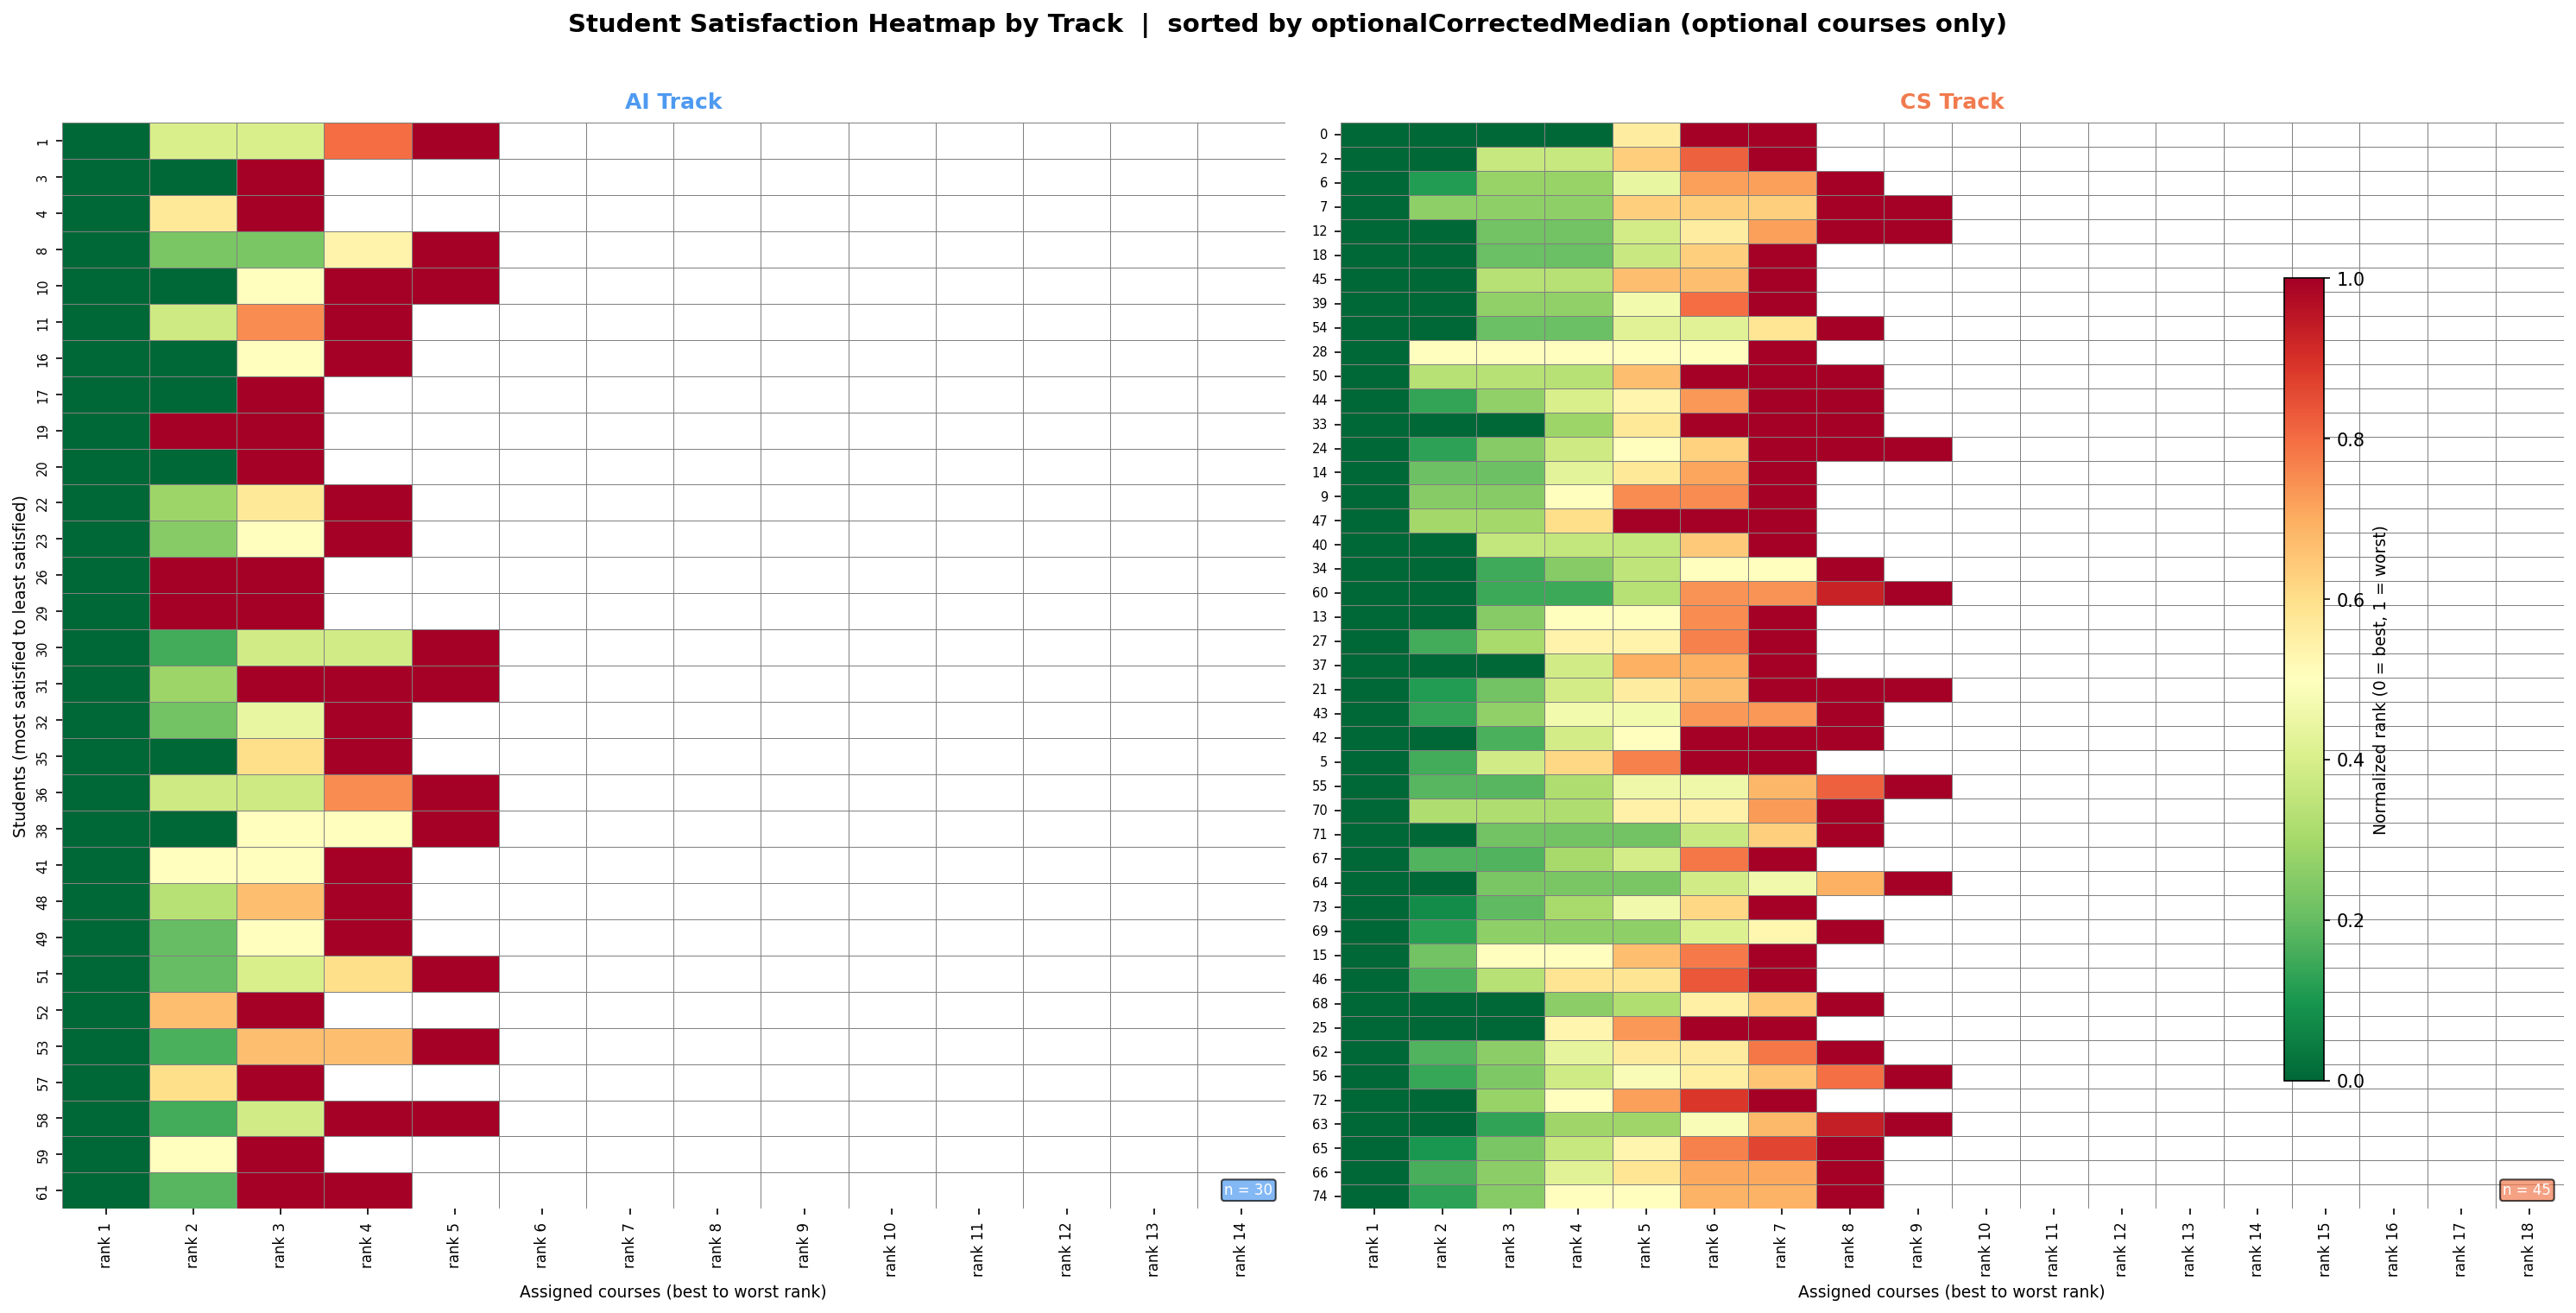
\includegraphics[width=\textwidth]{img/heatmapMedian.png}
    \caption{Heatmap des affectations}
\end{figure}

Sur ce tableau, les UEs obligatoires sont retirées, car elles ont le meilleur rang possible quoi qu'il arrive. De plus, comme les deux parcours n'ont pas nécessairement le même nombre d'UEs obligatoires, nous les séparons pour obtenir un résultat plus représentatif. Il ne reste donc plus que le rang normalisé à examiner.
Ainsi, nous pouvons comparer deux affectations à vue d'œil, en observant simplement laquelle est la plus << verte >>. Intuitivement, nous choisirons l'affectation qui satisfait le plus d'étudiants. À noter que cette visualisation peut changer en n'affichant qu'un parcours, en ne considérant pas de parcours en particulier, en remettant les UEs obligatoires ou en changeant l'ordre, qui est par défaut la médiane des rangs non facultatifs en ordre croissant.

L'objectif de ces visualisations n'est pas de remplacer le solveur, mais de rendre l'affectation \emph{auditable} et \emph{comparables} : on cherche à comprendre \emph{qui} est pénalisé et \emph{pourquoi}, et à quantifier les compromis utilité/équité entre différentes solutions.
Pour ce faire, regrouper les métriques vectorielles, certains indicateurs et graphiques dans un tableau de bord pourrait également être une bonne option. Nous pouvons aisément imaginer quelque chose comme ceci :
\begin{figure}[H]
    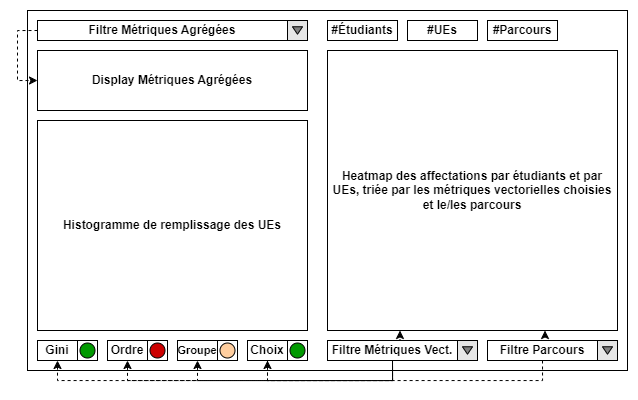
\includegraphics[width=\textwidth]{img/Dashboard UI Diagram.drawio.png}
    \caption{Schéma conceptuel d'un tableau de bord hypothétique}
\end{figure}
Où nous pourrions facilement accéder à toutes les métriques agrégées par un filtre, à l'histogramme de remplissage des UEs/leurs saturations, à des tests d'hypothèses sur l'ordre, le parcours ou le nombre d'UE choisies, ainsi qu'à l'indice de Gini si une affectation présente des propriétés non souhaitables sur des métriques choisies (indiquées par des pastilles de couleur verte, jaune ou rouge, par exemple). Nous pourrions également consulter les paramètres de notre affectation, ainsi que la heatmap de l'affectation des étudiants aux UEs en fonction du parcours et triée par la métrique choisie.

Ce tableau de bord n'a malheureusement pas pu être réalisé en raison de contraintes de temps.

\section{Conclusions}
En conclusion, ce projet vise à proposer un mécanisme d'affectation plus << satisfaisant >> que le système en place : << premier arrivé, premier servi >>, le tout en restant interprétable (au mieux explicable), en introduisant la notion d'équité et en la différenciant avec d'autres notions tels que l'optimalité ou l'intégrité.

Pour cela, le format des données a d'abord été formalisé, de même que les contraintes. Les notions d'équité et d'optimalité ont été étudiées en profondeur afin de déterminer les métriques et les objectifs les plus proches de ce que l'on considère comme une affectation << satisfaisante >>.
Dans un second temps, un modèle linéaire dont l'objectif est sélectionnable a été créé et utilisé au sein d'un solveur exact (OPL/CPLEX). Les affectations sortantes (au format CSV) sont ensuite analysées à l'aide des métriques précitées, puis visualisées afin de soutenir une décision d'affectation finale pour les étudiants.

L'approche présente deux atouts majeurs : d'une part, la faisabilité est garantie par construction lorsque le modèle admet une solution ; d'autre part, la séparation \og solveur \textrightarrow{} exports CSV \textrightarrow{} métriques/visualisations \fg{} permet de conserver un modèle d'optimisation simple, tout en offrant un espace riche d'évaluation a posteriori (Section~\ref{sec:Metric}).

\paragraph{Contributeurs} Les contributeurs aux projets sont les suivants :
Arezzoug Mounia (Entrée, génération pondérée),
Claveille Hugo (Entrée, Gestion de projet, gestion du git),
Cuvilliez Fiona (Entrée, génération uniforme, lien solveur),
Frelat Jade (Entrée, génération uniforme),
Andre Mathis (Solveur),
De Chabannes Curton La Palice Antoine (Solveur, formalisation des objectifs),
Levesque Du Rostu Mathis (Solveur),
Thiery Nathan (Solveur, modélisation et implémentation OPL/CPLEX),
Viana Hugo (Formalisation du problème, Gestion de projet),
Dogan Yunus Emre (Sortie, visualisation),
Lesage Arno (Formalisation du problème, Sortie, Rapport, formalisation des métriques),
Radi Youness (Sortie),
Lang Thomas (Présentation),
Hoàng Minh Quân (Gestion de projet, gestion du git),
Di Russo Marc (Rapport),
Malapert Arnaud (Gestion de projet, coordinateur, reviewer).

\bibliographystyle{plain}
\bibliography{refs.bib}

\end{document}
